\subsection*{g. Obtener el modo de envío y categoría que más productos ha vendido.}

Primero realizamos un join natural entre la tabla \textit{orders} y la tabla \textit{products} (comparten productid) para poder asociar las cantidades (\textit{quantity}), los modos de envío (\textit{shipmode}) y las categorías (\textit{category}). Después, aplicamos una operación $\gamma$ para agrupar por \textit{shipmode} y \textit{category}, y le aplicamos la función de agregación SUM a la cantidad de productos (\textit{quantity}), nombrando este valor agregado como \textit{TotalQty}. Llamaremos a esta relación $T$. Luego, sobre $T$ calculamos el valor máximo de estos totales (\textit{MaxQty}), realizando una nueva agrupación. A este resultado lo llamaremos $T_{max}$. Finalmente, cruzamos $T$ con $T_{max}$ (haciendo match donde \textit{TotalQty} sea igual a \textit{MaxQty}) y proyectamos únicamente los atributos \textit{shipmode} y \textit{category}.

Expresión:
\begin{equation}
\begin{split}
T &= \gamma_{shipmode,\, category;\, \text{SUM}(quantity) \rightarrow TotalQty}(orders \bowtie products) \\
T_{max} &= \gamma_{\text{MAX}(TotalQty) \rightarrow MaxQty}(T) \\
\text{Resultado} &= \pi_{shipmode,\, category}(T \bowtie_{TotalQty = MaxQty} T_{max})
\end{split}
\end{equation}

Resultados obtenidos:

\begin{figure}[h!]
\centering
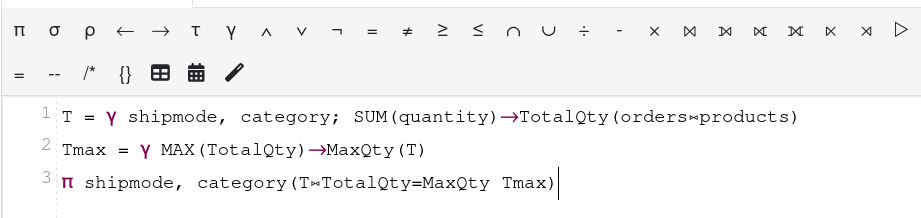
\includegraphics[width=0.8\textwidth]{imagenes/2g(1).png}
\caption{Consulta 2g.}
\end{figure}

\begin{figure}[h!]
\centering
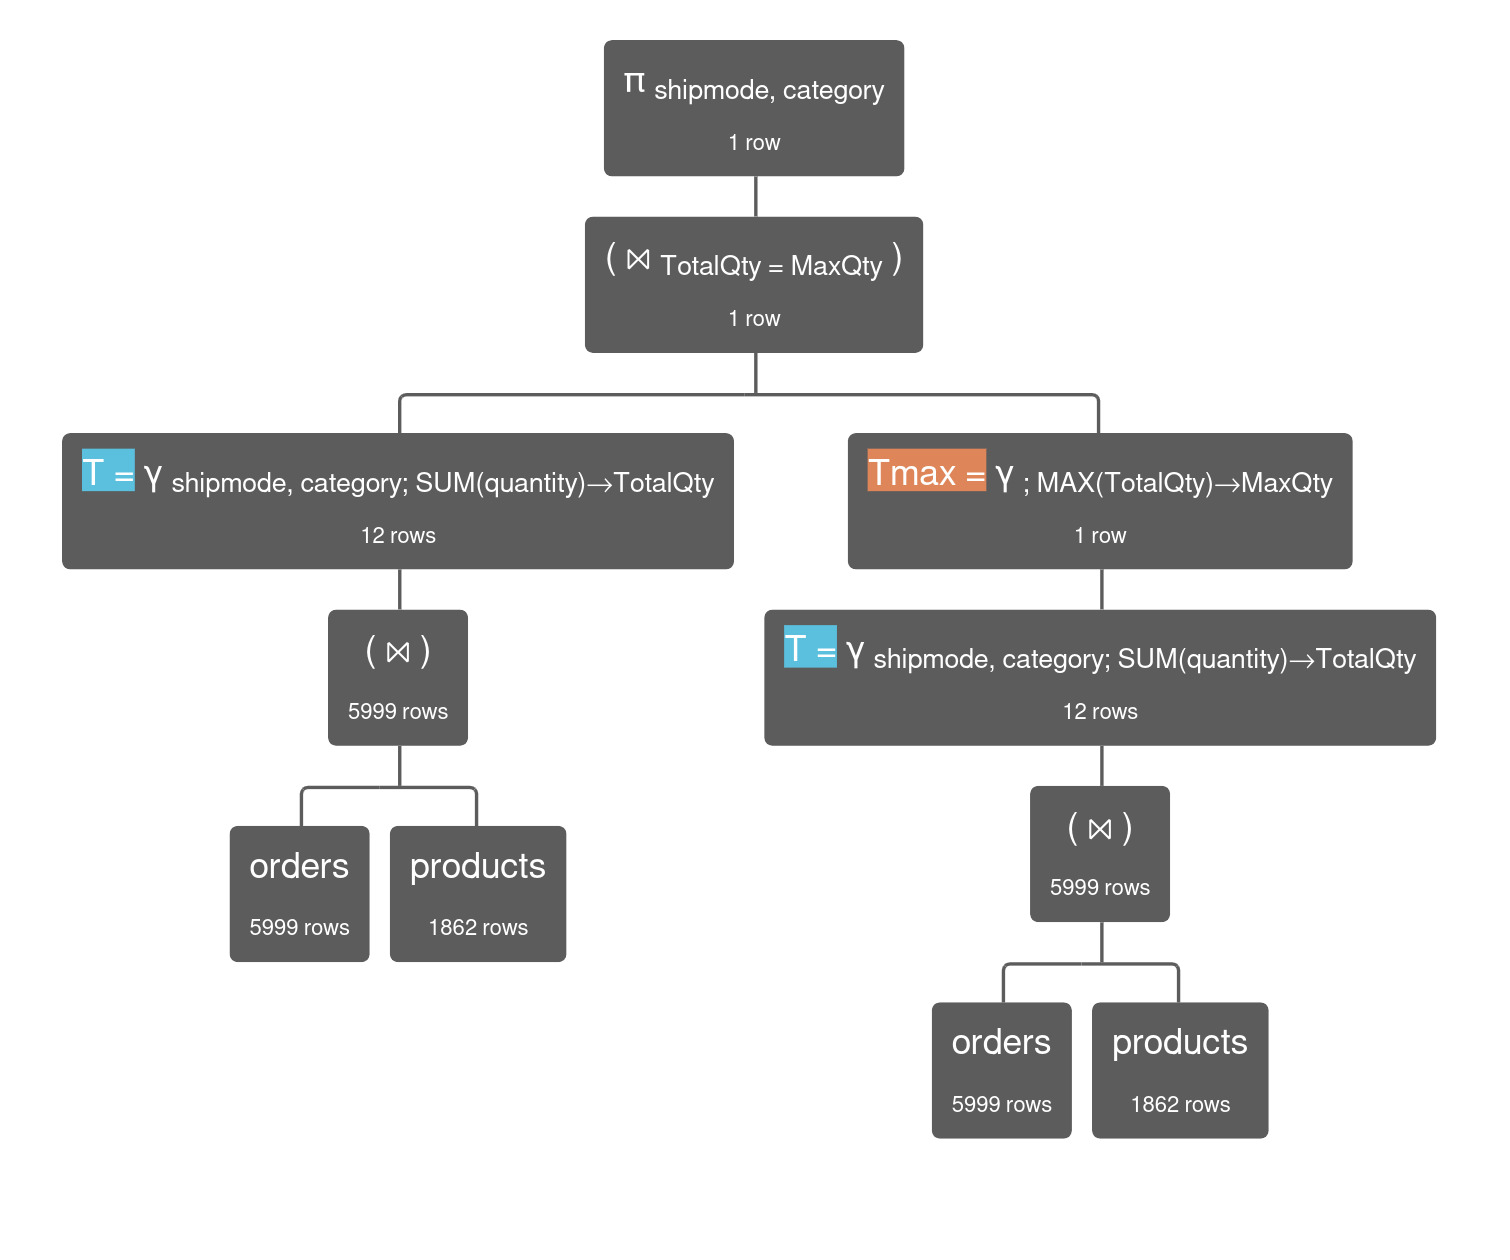
\includegraphics[width=0.8\textwidth]{imagenes/2g(2).png}
\caption{Árbol de consulta 2g.}
\end{figure}

\begin{figure}[h!]
\centering
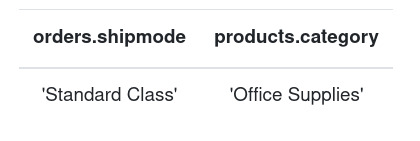
\includegraphics[width=0.8\textwidth]{imagenes/2g(3).png}
\caption{Resultado de consulta 2g.}
\end{figure}
